\documentclass[../../main.tex]{subfiles}

\graphicspath{{\subfix{../../immagini/}}}

\begin{document}
    Obiettivo di questo capitolo è di fornire una breve introduzione ai concetti fondamentali dell'apprendimento autmatico con un interesse particolare per i concetti di \textit{apprendimento supervisionato} e, nello specifico, alla \textit{classificazione} e alla \textit{regressione}.

    Inizio fornendo una formalizzazione del concetto di \textit{apprendimento} in ambito informatico:
    
    Data una classe di problemi $T$ ed un metodo di misura delle prestazioni $P$ si dice che un generico programma \textit{apprende} dall'esperienza accumulata in $T$ se le sue prestazioni, misurate tramite $P$, migliorano all'aumentare dell'esperienza $E$. \cite{Mitchell97}

    Nel contesto dei nostri esperimenti, ad esempio, il problema $T$ è quello di classificare correttamente, come phishing o sani, degli URL forniti in ingresso; il programma migliorerà le proprie prestazioni $P$, misurate come abilità di discernere correttamente URL, grazie all'esperienza  $E$ guadagnata tramite l'osservazione di un elevato numero di URL di entrambe le categorie, \textit{imparando} poi a generalizzare le caratteristiche principali di entrambe le tipologie di indirizzi e riuscendo infine a classificare correttamente nuovi URL mai osservati in precedenza.


    In generale quindi posso definire un problema di apprendimento identificando tre proprietà: la classe del problema, la metrica per le prestazioni e la fonte dell'esperienza.

    Identficato un problema di apprendimento l'obiettivo è ora quello di definire un approccio per la progettazione di sistemi in grado di risolvere tali problemi.\\
    A tal proposito è utile introdurre il concetto di \textit{agente}, che può essere definito come un'entità in grado di percepire l'ambiente tramite sensori e di interagire con tale ambiente tramite degli attuatori, potrò definire diverse tipologie di agente a seconda di come questo lavora sulle percezioni ottenute dall'ambiente.

    \begin{wrapfigure}{l}{0.5\textwidth}
        \begin{center}
            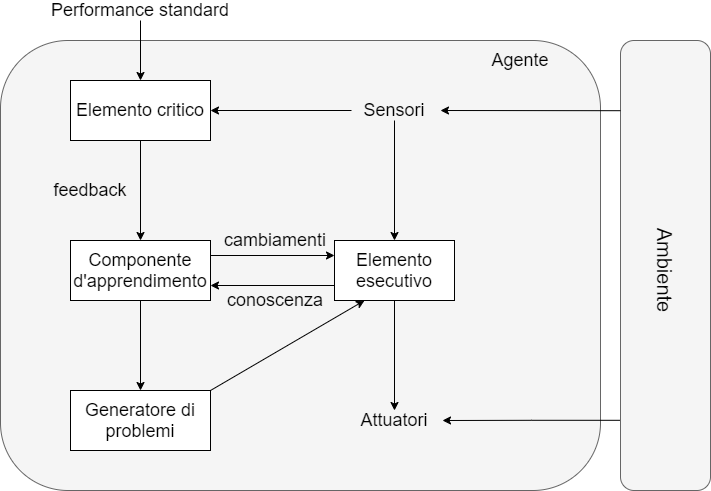
\includegraphics[width = 0.48\textwidth]{immagini/4_0/learning_agent.png}
        \end{center}
        \caption{Schema di un learning agent \cite{russel2010}}
        \label{fig:learning_agent}
    \end{wrapfigure}

    Nello specifico la tipologia di agente utilizzata nell'ambito dell'apprendimento automatico è quella che prende il nome di \textit{learning agent} (Figura \ref{fig:learning_agent}). Agenti di questo tipo possono essere suddivisi in quattro componenti principali di cui i due più importanti sono il \textit{learning element}, il cui compito è di migliorare le prestazioni dell'agente, ed il \textit{performance element}, il cui compito è di scegliere le azioni da compiere sulla base delle percezioni dall'ambiente; il learning element quindi migliora l'agente, sulla base del feedback ricevuto dal componente \textit{critic}, modificando il comportamento del performance element.

    Si dice quindi che un agente \textit{apprende} se le sue performance vanno a migliorare grazie a ripetute interazioni con l'ambiente in cui è inserito.
    Importante notare come il concetto di agente sia applicabile in generale a tutti i campi dell'intelligenza artificiale, non solo a quello del \textit{machine learning}, trattato in questo capitolo.

    Posso definire diverse forme di apprendimento a seconda di come i vari componenti dell'agente vengono caratterizzati, nello specifico concentrandosi sulla tipologia di feedback ricevuto dall'agente vengono determinati le tre principali forme di apprendimento:

    \textit{Apprendimento supervisionato}: in questo caso l'agente apprende tramite un dataset di esempi, in cui ogni esempio è nella forma $<input, output>$.

    \textit{Apprendimento non supervisionato}: a differenza di ciò che accade nel caso precendente, in questo contesto l'agente riesce ad apprendere senza avere un feedback con cui confrontare le proprie assunzioni. Esempio classico di apprendimento di questo tipo è il \textit{clustering}.

    \textit{Apprendimento per rinforzo}: l'agente apprende tramite una serie di \textit{reward} o \textit{punishment}.

    È importante sottolineare come seppur l'apprendimento per rinforzo sia spesso presentato come uno dei tipi di apprendimento insieme agli altri due in realtà non è del tutto comparabile: molte tecniche classificabili come di apprendimento supervisionato, ad esempio, possono essere sfruttate nel contesto dell'apprendimento per rinforzo (\textit{Regressione} $\rightarrow$ \textit{Q-learning}).

    Mi concentro ora sull'apprendimento supervisionato, che sarà la tipologia di apprendimento che sfrutterò negli esperimenti descritti in seguito.
    


\end{document}